\listfiles
\documentclass[12pt]{report}\usepackage[]{graphicx}\usepackage[]{color}
%% maxwidth is the original width if it is less than linewidth
%% otherwise use linewidth (to make sure the graphics do not exceed the margin)
\makeatletter
\def\maxwidth{ %
  \ifdim\Gin@nat@width>\linewidth
    \linewidth
  \else
    \Gin@nat@width
  \fi
}
\makeatother

\usepackage{Sweavel}



\usepackage[intoc]{nomencl}
\textwidth=6in \oddsidemargin=0.5in \topmargin=-0.5in
\textheight=9in  % 9in must include page numbers
\textfloatsep = 0.4in 
\addtocontents{toc}{\vspace{0.4in} \protect \hfill Page\endgraf} 
\addtocontents{lof}{\vspace{0.2in} \hspace{0.13in} \ Figure \protect \hfill Page\endgraf} \addtocontents{lot}{\vspace{0.2in} \hspace{0.13in} \ Table \protect\hfill Page\endgraf}

%%%%%%%%%%%%%%%%%%%%%%%%%%%%%%%
%-------------- USE PACKAGE-----------------------------------------%
%%%%%%%%%%%%%%%%%%%%%%%%%%%%%%%

%\usepackage[natbibapa]{apacite}
\usepackage{array}
\newcolumntype{L}{>{\centering\arraybackslash}m{5cm}}
\newcolumntype{R}{>{\centering\arraybackslash}m{2cm}}

\usepackage{amsmath}
\usepackage{mathtools}
\usepackage{longtable}
\usepackage{graphicx}
\usepackage{multirow}
\usepackage[font=singlespacing]{caption}
%\usepackage{caption}
%\captionsetup{font=scriptsize}
\captionsetup{font=footnotesize}
\usepackage[nottoc,notlof,notlot]{tocbibind}
\renewcommand\bibname{REFERENCES}
%\usepackage[backend=bibtex,style=verbose-trad2]{biblatex}
%\bibliography{/Users/mollyolson/Documents/Vanderbilt/Masters_Thesis/ThesisWork/thesisBib.bib}

%\usepackage{cite}


\usepackage{setspace}
\usepackage{titlesec}
\usepackage{tgschola}
\usepackage{color}
\usepackage[left=1.5in,right=1in,top=1in,bottom=1in]{geometry}
\usepackage[table]{xcolor}
 \usepackage{amsfonts}
 \usepackage{amsmath}
 \usepackage{amsbsy,bm}
 \usepackage{amssymb}
\usepackage{graphicx}
 \usepackage{setspace}
 \usepackage{rotating}
 \usepackage{float}
 \usepackage{stmaryrd}
 \usepackage{multirow}
 \usepackage{color}
 \usepackage{soul}
 \usepackage{caption}
\usepackage{eepic}
\usepackage{colortbl}
%\usepackage[numbers]{natbib}
%\usepackage{natbib}
%\usepackage{natbib}
%\setcitestyle{citesep={;}, aysep={,}}
\newcommand\harvardand{\&}

%\renewcommand{\bibname}{References}




\usepackage{multirow}
\usepackage{setspace}
\usepackage{indentfirst}
\usepackage{titlesec}
\usepackage{subfig}
\usepackage[mathscr]{euscript}
\usepackage[titletoc,title]{appendix}
\usepackage[titletoc]{appendix}
\usepackage[tocgraduated]{tocstyle}

\usepackage{textcomp}
\usepackage{array}
\usepackage{listings}
\usepackage{setspace}
\usepackage{mathptmx}
\usepackage{colortbl}
\usepackage{graphicx}
\usepackage{amssymb, amsmath}
\usepackage{subfig}
\usepackage{epsfig}
\usepackage{times}
\usepackage{float}
\usepackage{rotating}
\usepackage{makeidx}
\usepackage{url}
\usepackage{multirow}
\usepackage{booktabs}
\usepackage[subfigure, titles]{tocloft}
\usepackage[hidelinks]{hyperref}

\usepackage{acronym}
\usepackage{datetime}
\usepackage{algorithm}
\usepackage{algorithmic}
\usepackage{url, hyperref}
%\usepackage{cleveref}
\renewcommand{\nomname}{LIST OF ABBREVIATIONS}
\makenomenclature
\graphicspath{{images/}}
\DeclareGraphicsExtensions{.pdf,.jpeg,.png,.PNG, .eps, .tiff}

\urlstyle{same}

\usepackage{makecell}
\usepackage{titletoc}
\usepackage{appendix}
\usepackage[nottoc]{tocbibind}
\setcounter{secnumdepth}{7}
\setcounter{tocdepth}{7}
\usepackage{lscape}

\DeclarePairedDelimiter\ceil{\lceil}{\rceil}
\DeclarePairedDelimiter\floor{\lfloor}{\rfloor}

%%%%%%%%%%%%%%%%%%%%%%%%%%%%%%%
%-------------- NEW COMMANDS-------------------------------------%
%%%%%%%%%%%%%%%%%%%%%%%%%%%%%%%
%new chapter/section and subsection commands
\newcommand{\hsuchapter}[1]{\chapter*{#1} \addcontentsline{toc}{chapter}{#1} } 
\newcommand{\hsusection}[1]{\section*{#1} \addcontentsline{toc}{section}{#1} } 
\newcommand{\hsusubsection}[1]{\subsection*{#1} \addcontentsline{toc}{subsection}{#1} } 

%%%%%%%Configure Table of Contents%%%%%%%%%%%%
\renewcommand{\contentsname}{TABLE OF CONTENTS}
\renewcommand{\cftchapfont}{\normalfont}
\renewcommand{\cftchappagefont}{\normalfont}
\renewcommand{\cftchapleader}{\cftdotfill{\cftdotsep}}

%%%%%%%Configure List of Figures%%%%%%%%%%%%
\renewcommand{\listfigurename}{LIST OF FIGURES}
\setlength{\cftbeforefigskip}{0.2in}

%%%%%%%Configure List of Tables%%%%%%%%%%%%
\renewcommand{\listtablename}{LIST OF TABLES}
\setlength{\cftbeforetabskip}{0.2in}

%%%%%% Configure ABSTRACT %%%%%%
\usepackage{abstract}
\renewcommand{\abstractname}{ABSTRACT}




%%%%%%%Configure Bibliography%%%%%%%%%%%%
\renewcommand{\bibname}{ \texorpdfstring{{REFERENCES\vspace{10mm}}}{REFERENCES}   }

%%%%%%%%%%%%%%%%%%%%%%%%%%%%%%%
%-------------- CONFIGURE CHAPTER HEADINGS--------------%
%%%%%%%%%%%%%%%%%%%%%%%%%%%%%%%



\makeatletter
\def\@makechapterhead#1{
  {\parindent \z@ %\centering
    \LARGE \fontfamily{qcs}\selectfont
    \ifnum \c@secnumdepth >\m@ne
      \if@mainmatter
        \@chapapp\space \thechapter
        \par\nobreak
        \vskip 20\p@
      \fi
    \fi
    \interlinepenalty\@M
    #1\par\nobreak
    \vskip 40\p@
  }}
\def\@schapter#1{\if@twocolumn
                   \@topnewpage[\@makeschapterhead{#1}]%
                 \else
                   \@makeschapterhead{#1}%
                   \@afterheading
                 \fi}
\def\@makeschapterhead#1{
  {\parindent \z@ \centering
    \large
    \interlinepenalty\@M
    #1\par\nobreak
    \vskip 10\p@
  }}




%%% this configure the linespace in the table of content
%%% code is complicated and ugly but it works
\newlength{\li}\setlength{\li}{14.48pt}
\newlength{\di}\setlength{\di}{-3.5mm}
\def\@chapter[#1]#2{\ifnum \c@secnumdepth >\m@ne
      \refstepcounter{chapter}%
      \typeout{\@chapapp\space\thechapter.}%
      \addcontentsline{toc}{chapter}{\numberline{\thechapter}#1}
         %{\protect\numberline{\thechapter}\uppercase{#1}}%
      \addtocontents{toc}{\protect\vspace{\li}}%
  \else
      %\addcontentsline{toc}{chapter}{\uppercase{#1}}%
      \addcontentsline{toc}{chapter}{#1}
      \addtocontents{toc}{\protect\vspace{\li}}%
  \fi
  \chaptermark{#1}%
  \if@twocolumn
      \@topnewpage[\@makechapterhead{#2}]%
  \else
      \@makechapterhead{#2}%
      \@afterheading
 \fi}


\renewcommand\chapter{\addtocontents{toc}{\protect\addvspace{\li}}%
  \if@openright\cleardoublepage\else\clearpage\fi
  \thispagestyle{plain}%
  \global\@topnum\z@
  \@afterindentfalse
  \secdef\@chapter\@schapter}

%%%%%%%%%%%%%%%%%%%%%%%%%%%%%%%%%%%%%%%%%%%%%%%%%%%%%%%%%%%%%%
%-----------CONFIGURE SECTION HEADINGS------------------%
%%%%%%%%%%%%%%%%%%%%%%%%%%%%%%%%%%%%%%%%%%%%%%%%%%%%%%%%%%%%%%
\renewcommand\section{ \@startsection {section}{1}{\z@}%
                                   {-3.5ex \@plus -1ex \@minus -.2ex}%
                                   {2.3ex \@plus.2ex}%
                                   {\centering\large\fontfamily{qcs}\selectfont}}


                    
%%%%%%%%%%%%%%%%%%%%%%%%%%%%%%%%%%%%%%%%%%%%%%%%%%%%%%%%%%%%%%
%-------------CONFIGURE SUBSECTION HEADINGS- --------%
%%%%%%%%%%%%%%%%%%%%%%%%%%%%%%%%%%%%%%%%%%%%%%%%%%%%%%%%%%%%%%
\renewcommand\subsection{\@startsection {subsection}{2}{\z@}%
                                   {-3.5ex \@plus -1ex \@minus -.2ex}%
                                   {2.3ex \@plus.2ex}%
                                   {\noindent \large \fontfamily{qcs}\selectfont }}
                                  
      
                                   

%%%%%%%Sub-Sub-Section's Not  Supported%%%%%%%%%%%%

%%%%%%%%%%%%%%%%%%%%%%%%%%%%%%%%%%%%%%%%%%%%%%%%%%%%%%%%%%%%%%
%-------CONFIGURE TABLE OF CONTENTS HEADING------%
%%%%%%%%%%%%%%%%%%%%%%%%%%%%%%%%%%%%%%%%%%%%%%%%%%%%%%%%%%%%%%
\renewcommand{\@cftmaketoctitle}{
  \chapter*{\contentsname}
  \addcontentsline{toc}{chapter}{TABLE OF CONTENTS}} 

%%%%%%%%%%%%%%%%%%%%%%%%%%%%%%%%%%%%%%%%%%%%%%%%%%%%%%%%%%%%%%
%------CONFIGURE LIST OF FIGURES HEADING------------%
%%%%%%%%%%%%%%%%%%%%%%%%%%%%%%%%%%%%%%%%%%%%%%%%%%%%%%%%%%%%%%
\renewcommand{\@cftmakeloftitle}{
  \chapter*{\listfigurename}
  Figure \hfill Page
  \addcontentsline{toc}{chapter}{LIST OF FIGURES} } 
  
%%%%%%%%%%%%%%%%%%%%%%%%%%%%%%%%%%%%%%%%%%%%%%%%%%%%%%%%%%%%%%
%--------CONFIGURE LIST OF TABLES HEADING-------------%
%%%%%%%%%%%%%%%%%%%%%%%%%%%%%%%%%%%%%%%%%%%%%%%%%%%%%%%%%%%%%%
\renewcommand{\@cftmakelottitle}{
  \chapter*{\listtablename}
   Table \hfill Page
   \addcontentsline{toc}{chapter}{LIST OF TABLES} }  

\makeatother

\setcounter{section}{-1}     

%%%%%%%%%%%%%%%%%%%%%%%%%%%%%%%%%%%%%%%%%%%%%%%%%%%%%%%%%%%%%%
%---------------------------NEW COMMANDS-------------------------%
%%%%%%%%%%%%%%%%%%%%%%%%%%%%%%%%%%%%%%%%%%%%%%%%%%%%%%%%%%%%%%
\newcommand{\etal}{\emph{et al.}}
\newcommand{\leftsup}[2]{{\vphantom{#2}}^{#1}{#2}}
\newcommand{\leftsub}[2]{{\vphantom{#2}}_{#1}{#2}}
\newcommand{\leftsupsub}[3]{{\vphantom{#3}}^{#1}_{#2}{#3}}

\DeclareMathOperator*{\assembly}{\textbf{\Large A} }

\definecolor{lightblue}{rgb}{.90,.95,1} 
\newcommand{\hllb}[1]{
	\sethlcolor{lightblue}
	\hl{#1}
	\sethlcolor{yellow}
	}

\newcommand{\hlc}[2][yellow]{{\sethlcolor{#1}\hl{#2}} }

%%%%%%%%%%%%%%%%%%%%%%%%%%%%%%%%%%%%%%%%%%%%%%%%%%%%%%%%%%%%%%
%--------------DEFINE FLOATS----------------------------------------%
%%%%%%%%%%%%%%%%%%%%%%%%%%%%%%%%%%%%%%%%%%%%%%%%%%%%%%%%%%%%%%
 \floatstyle{plain}
 \newfloat{Box}{h}{lob}
 \newcommand{\boxedtext}[3]{
 	\begin{Box} \caption{\small{#1}}
	\hspace{1.cm}
	\fbox{\begin{minipage}[c]{0.85\linewidth} 
	
	\small{#2}
       
       \end{minipage}}
       
       \label{#3}
       \end{Box}
  }

 \begin{document}


%\pagestyle{myheadings} \markright{\today}
%%%%%%%%%%%%%%%%%%%%%%%%%%%%%%%%%%%%%%%%%%%%%%%%%%%%%%%%%%%%%%
%-------------- MAKE TITLE CHANGES HERE---------------------%
%%%%%%%%%%%%%%%%%%%%%%%%%%%%%%%%%%%%%%%%%%%%%%%%%%%%%%%%%%%%%%
\pagenumbering{alph}

\begin{titlepage}
\thispagestyle{empty}\enlargethispage{\the\footskip}%
\begin{center}
	{\setstretch{1.66} {Working Title: A Comparison of Approaches for Unplanned Sample Sizes in Phase II Clinical Trials}\par }%
	\vskip.4in
	By
	\vskip .3in
	{Molly Olson}
	\vskip .3in
	
	\begin{doublespace}
	Thesis\\
		Submitted to the Faculty of the \\
		Graduate School of Vanderbilt University \\
		in partial fulfillment of the requirements \\
		for the degree of \\ [.1in]
	\end{doublespace}
	
	\MakeUppercase{MASTER OF SCIENCE} \\[.1in]
	in \\[.1in]
	{Biostatistics} \\[.25in]
	May, 2017 \\[.25in]
	Nashville, Tennessee
	\vskip .5in
%\end{center}
%%%Uncomment for Signatures%%%
%Approved: \hskip 2.9in Date:\\[1.2em]
%\rule{3.5in}{.5pt} \hskip 0.1in \rule{2in}{.5pt} \\[.01in]
%Professor John D. Doe \\[.14in]
%\rule{3.5in}{.5pt} \hskip 0.1in \rule{2in}{.5pt}  \\[.01in]
%Professor John D. Doe \\[.14in]
%\rule{3.5in}{.5pt} \hskip 0.1in \rule{2in}{.5pt} \\[.01in]
%Professor John D. Doe \\[.14in]
%\rule{3.5in}{.5pt} \hskip 0.1in \rule{2in}{.5pt} \\[.01in]
%Professor John D. Doe \\[.14in]
%\\[.14in]
%%%%%%%%%%%%%%
%%%%%%Uncomment  for Approved Names%%%%%%
\begin{doublespace}
Approved (in progress):\\
Tatsuki Koyama , Ph.D. \\
Jeffrey Blume , Ph.D. \\
\end{doublespace}
%%%%%%%%%%%%%%%%%%%%%%%%%%%%%%%%%%%%%%%
\end{center}
\end{titlepage}
 
\doublespacing
\pagenumbering{roman} \setcounter{page}{2}

%\chapter*{The dedication page is optional. If you don't use it, please delete it.}
%\addcontentsline{toc}{chapter}{DEDICATION}
%\vspace{7mm}

%%%%%%%%%%%%%%%%%%%%%%%%%%%%%%%%%%%%%%%%%%%%%%%%%%%%%%%%%%%%%%
%--------------ACKNOWLEDGEMENTS----------- -----------------%
%%%%%%%%%%%%%%%%%%%%%%%%%%%%%%%%%%%%%%%%%%%%%%%%%%%%%%%%%%%%%%
\chapter*{ACKNOWLEDGMENTS}
\addcontentsline{toc}{chapter}{ACKNOWLEDGMENTS}
\vspace{7mm}


%%%%%%%%%%%%%%%%%%%%%%%%%%%%%%%%%%%%%%%%%%%%%%%%%%%%%%%%%%%%%%
%-------------- BEGIN TABLE OF CONTENTS---------------------%
%%%%%%%%%%%%%%%%%%%%%%%%%%%%%%%%%%%%%%%%%%%%%%%%%%%%%%%%%%%%%%
\begin{singlespace}
\tableofcontents
\newpage
\addcontentsline{toc}{chapter}{\listtablename}
\end{singlespace}

%%%%%%%%%%%%%%%%%%%%%%%%%%%%%%%%%%%%%%%%%%%%%%%%%%%%%%%%%%%%%%
%--------------BEGIN LIST OF TABLES------------------------------%
%%%%%%%%%%%%%%%%%%%%%%%%%%%%%%%%%%%%%%%%%%%%%%%%%%%%%%%%%%%%%%
\listoftables

%%%%%%%%%%%%%%%%%%%%%%%%%%%%%%%%%%%%%%%%%%%%%%%%%%%%%%%%%%%%%%
%--------------BEGIN LIST OF FIGURES----------------------------%
%%%%%%%%%%%%%%%%%%%%%%%%%%%%%%%%%%%%%%%%%%%%%%%%%%%%%%%%%%%%%%
\newpage
\addcontentsline{toc}{chapter}{\listfigurename}
\listoffigures
\newpage
%%%%%%%%%%%%%%%%%%%%%%%%%%%%%%%%%%%%%%%%%%%%%%%%%%%%%%%%%%%%%%
%-------------- ABSTRACT-----------------------------------------------%
%%%%%%%%%%%%%%%%%%%%%%%%%%%%%%%%%%%%%%%%%%%%%%%%%%%%%%%%%%%%%%
\addcontentsline{toc}{chapter}{ABSTRACT}
\chapter*{ABSTRACT}

\vspace{7mm}
In this thesis, we develop .....
\newpage

\normalsize
\doublespacing
\pagenumbering{arabic}
\setcounter{page}{1}
%%%%%%%%%%%%%%%%%%%%%%%%%%%%%%%%%%%%%%%%%%%%%%%%%%%%%%%%%%%%%%%%%%%%%%%%%%%%%%%%%%%%%%%%%%%%%%%%%%%%%%%%%%%%%%%%%%
%%%%%%%%%%%%%%%%%%%%%%%%%%%%%%%%%%%%%%%%%%%%%%%%%%%%%%%%%%%%%%%%%%%%%%%%%%%%%%%%%%%%%%%%%%%%%%%%%%%%%%%%%%%%%%%%%%
%%%%%%%%%%%%%%%%%%%%%%%%%%%%%%%%%%%%%%%%%%%%%%%%%%%%%%%%%%%%%%%%%%%%%%%%%%%%%%%%%%%%%%%%%%%%%%%%%%%%%%%%%%%%%%%%%%
%%%%%%%%%%%%%%%%%%%%%%%%%%%%%%%%%%%%%%%%%%%%%%%%%%%%%%%%%%%%%%%%%%%%%%%%%%%%%%%%%%%%%%%%%%%%%%%%%%%%%%%%%%%%%%%%%%
%% -----------------------------------WRITING STARTS HERE ------------------------------------------------------%%
%%%%%%%%%%%%%%%%%%%%%%%%%%%%%%%%%%%%%%%%%%%%%%%%%%%%%%%%%%%%%%%%%%%%%%%%%%%%%%%%%%%%%%%%%%%%%%%%%%%%%%%%%%%%%%%%%%
%%%%%%%%%%%%%%%%%%%%%%%%%%%%%%%%%%%%%%%%%%%%%%%%%%%%%%%%%%%%%%%%%%%%%%%%%%%%%%%%%%%%%%%%%%%%%%%%%%%%%%%%%%%%%%%%%%
%%%%%%%%%%%%%%%%%%%%%%%%%%%%%%%%%%%%%%%%%%%%%%%%%%%%%%%%%%%%%%%%%%%%%%%%%%%%%%%%%%%%%%%%%%%%%%%%%%%%%%%%%%%%%%%%%%
%%%%%%%%%%%%%%%%%%%%%%%%%%%%%%%%%%%%%%%%%%%%%%%%%%%%%%%%%%%%%%%%%%%%%%%%%%%%%%%%%%%%%%%%%%%%%%%%%%%%%%%%%%%%%%%%%%


%---------------------------------------------------------------------------------------------------------------%
%------------------------------------------------CHAPTER1------------------------------------------------%
%---------------------------------------------------------------------------------------------------------------%

%% comparison by itself is interesting
%% chang et al design is a little bit better - it's a new contribution so it won't feel like it's only reviews. 
%% make sure that comes out in the paper
%% maybe change the section title

%%%%%%%%%%%%%%%%%%%%%%%%%%%%%%%%%%%%%%%%%%%%%%%%%%%%%%%%%%%%%%
%------------Introduction------------------------------------%
%%%%%%%%%%%%%%%%%%%%%%%%%%%%%%%%%%%%%%%%%%%%%%%%%%%%%%%%%%%%%%
\cftlocalchange{toc}{450pt}{0cm}
\cftaddtitleline{toc}{chapter}{Chapter}{}
\cftlocalchange{toc}{1.55em}{2.55em}
\chapter{Introduction}
\vspace{-7mm}
The introduction will talk about the motivation for the thesis. Introduce some examples of when we would need such methods. 
\newline
\newline

Oncology phase II clinical trials are often used to evaluate the initial effect of a new regimen to determine if to warrant further study in a phase III clinical trial \cite{Porcher, Simon, Koyama}. Simon's two-stage design \cite{Simon} is a commonly used design in specifying sample sizes and critical values in phase II oncology clinical trials. Koyama and Chen \cite{Koyama} point out that it is common for actual sample sizes of these phase II trials to differ than the planned, pre-specified sample sizes. This could happen because of unanticipated accruement speed, drop-out rates are unexpected, and often multi-center trials can be slow in sharing information ... Currently, when attained sample sizes differ from planned, call these unplanned sample sizes, it is common practice to treat the attained sample sizes as planned. Though, when acheived sample sizes differ from planned, hypothesis testing using the attained sample sizes as if they were planned is not valid and hypothesis testing in these cases is not straightforward \cite{Porcher, Koyama}. Because of these reasons, extensions of Simon's design for hypothesis testing with unplanned sample sizes is important. 
\newline
\textit{Talk about examples here}
\newline
There have been many attempts to develop Frequentist methods that handle unplanned sample sizes in the second stage while using the planned stage I sample size, but my literature review found that there were only few Frequentist methods to handle unplanned sample sizes in both stage I and stage II. Likelihood based designs, that are able to be an extension of Simon's design, offer a nice solution to this problem because these designs offer flexibility in sample size without inflation of type I error.  In this paper, we discuss the different methods for Simon's design when the attained stage II sample size is different than planned and when attained sample sizes in both stages are different than planned. In chapter 4, we review a concrete example from a Likelihood-based clinical trial, and in chapter 5, results of a numerical and theoretical study comparing the Frequentist properties of approaches in the setting where both stages differ \textbf{wording} in different settings are presented.    
%%%%%%%%%%%%%%%%%%%%%%%%%%%%%%%%%%%%%%%%%%%%%%%%%%%%%%%%%%%%%%
%-------------Background-------------------------------------%
%%%%%%%%%%%%%%%%%%%%%%%%%%%%%%%%%%%%%%%%%%%%%%%%%%%%%%%%%%%%%%
\chapter{Background}
\vspace{-7mm}

%------------------------------------------------------------%
%----------- Background on Simon's design -------------------%
%------------------------------------------------------------%
Simon's design will go here. This section will also talk about extending/shortening a trial (unplanned sample sizes) and how recalculating as if it were the planned design will introduce bias and inflate type I error. Talk about prespecifying (maybe here?)
\newline
We will only talk about extensions to Simon's design, hypothesis testing, and only stopping for futility in this paper.  
\newline
\textbf{}
\newline
\indent Simon's II stage designs for clinical trials are common designs for phase II oncology clinical trials \cite{Simon}. In Simon's designs, the null hypothesis $\mbox{H}_0: p \leq p_0$ is tested against the alternative $\mbox{H}_1: p > p_1$, where $p$ is the true response probability, $p_0$ is the highest probability of response that would indicate that the research regimen is uninteresting and $p_1$ is the lowest probability of response that would indicate that the research regimen warrents further investigation. Under these hypotheses, it is required that the type I error rate remain less than $\alpha$ and power remain above $1-\beta$. The general framework of Simon's design includes a sample size and critical value in each of the two stages. Let $n_1$ denote the first stage sample size, $n_t$ the sample size at the end of the second stage, $r_1$ the first stage critical value, and $r_t$ the critical value for the end of the second stage. Let $X_1$ be the number of successes observed in the first stage and $X_2$ be the number of additional success in the second stage. In the first stage, $n_1$ patients are enrolled. If $r_1$ or fewer patients ($X_1 \leq r_1$) are successes, then the regimen is rejected and the trial is stopped for futility. If $r_1 + 1$ patients are successful, then the trial continues to the second stage. In the second stage, $n_2 = n_t - n_1$ patients are enrolled. If $r_t$ or fewer out of the $n_t$ patients are successful ($X_t = X_1 + X_2 \leq r_t$), the treatment is considered to be futile, otherwise if $r_t + 1$ patients succeed, the treatment is considered to be effective and warrent further study.  \\
\indent Design characteristics: Let $B$ denote the cumulative binomial distribution function and $b$ denote the binomial probability mass function. The probability of early termination with probability $p$ in Simon's designs is given by PET = $B(r_1, p, n_1)$. The expected sample size for probability $p$ is then $\mbox{EN} = n_1 + (1-\mbox{PET})n_2$. The probability of rejecting a drug for probability $p$ is then  $PR(p) = B(r_1, p, n_1) + \sum_{x=r_1+1}^{min[n_1,r]} b(x, p, n_1) B(r-x,p,n_2)$. It is required that $PR(p) \geq 1-\alpha$ and $PR(p) \leq \beta$. Given these constraints, it follows that unconditional conditional power, $UCP(p)$, given probability $p$, is given by $1-PR(p) = 1 - \left( B(r_1, p, n_1) + \sum_{x=r_1+1}^{min[n_1,r]} b(x, p, n_1) B(r-x,p,n_2) \right) = \sum_{r_1+1}^{n_1} \left\{\sum_{x_2 = r_t-x_1+1}^{n_2} b(x_2, p, n_2) \right\} b(x_1, p, n_1)$, and $UCP(p_1) \geq 1-\beta$ and $UCP(p_0) \leq \alpha$. \\
\indent Simon introduced optimal and minimax designs. An optimal two-stage design is a Simon's design in which minimizes the expected sample size under the null hypothesis, response value $p_0$, ($\mbox{EN}_0$) while still satisfying the type I and type II error probability restrictions. The minimax design will minimize the maximum sample size ($n_1 + n_2$). Jung \textit{et al.} \cite{Jung} introduced an extension of Simon's designs called admissible designs that are considered a compromise between optimal and minimax designs because they have similar maximim sample size as the minimax design and a similar $EN_0$ to the optimal design.  Admissible designs optimize a straight line on the ($n$, $EN$)-plane, $q \times n + (1-q) \times \mbox{EN}$, for some $q \in [0,1]$ \cite{Jung}. Admissible designs satisfy ($\alpha, \beta$) constraints and obtain an expected sample size somewhere between optimal and minimax designs. Admissible designs may be attractive because they have agreeable properties of both the minimax and optimal design.  Simon does not allow for early termination of the trial for efficacy \cite{Simon}, and we do not consider that design here. 

\begin{itemize}
  \item We consider only redesigns here -something you can prespecify. Not calculate after you get the values. 
  \item Talk about this in the "why we care"
\end{itemize}

%%%%%%%%%%%%%%%%%%%%%%%%%%%%%%%%%%%%%%%%%%%%%%%%%%%%%%%%%%%%%%
%------------------Literature Review-------------------------%
\chapter{Deviation from Planned Sample Sizes}
%%%%%%%%%%%%%%%%%%%%%%%%%%%%%%%%%%%%%%%%%%%%%%%%%%%%%%%%%%%%%%
This chapter will talk about unplanned sample sizes when only the second stage is different and when both stages can be different. The former will talk about methods such as Koyama and Chen, UMVUE, MLE, etc. The latter will talk about the likelihood design, Chang, adaptation of Chang, and possibly Wu. 

%%%%%%%%%%%%%%%%%%%%%%%%%%%%%%%%%%%%%%%%%%%%%%%%%%%%%%%%%%%%%%%
%----------Unplanned sample size in the first stage-----------%
\section{Deviation from Planned Sample Sizes in Second Stage}
%%%%%%%%%%%%%%%%%%%%%%%%%%%%%%%%%%%%%%%%%%%%%%%%%%%%%%%%%%%%%%%%

When over- or under-enrollment occurs, a straightforward solution is to perform an interim analysis on the planned number of first stage subjects, and adjust the testing procedure for a sample size in the second stage that is different than planned. This is possible under the assumption of non-informative dropouts; stage one is concluded when the number of non-missing patients is equal to the planned stage one sample size, and if over enrollment occurs in the first stage, they will only be considered for the second stage analysis \cite{Koyama}. Literature exists describing point estimation of the response rate and p-values for hypothesis testing when stage two sample size is modified. A review of these methods can be found by Porcher et al. \cite{Porcher}. Because, Koyama and Chen have shown that the p-value in multistage trials will depend on the design and is complicated in the setting of unplanned sample sizes \cite{Koyama} and our intent to pre-specify redesigned trials, we only focus on methods that use critical values for hypothesis testing and will not focus on p-value calculations. \textbf{(Basically calculating a p-value is complicated in unplanned settings, so we are just going to use critical values instead)} Koyama et al. propose a method for inference when stage II sample sizes deviate from the planned stage II sample size \cite{Koyama}. Let $n_1, n_t, r_1, r_t, \alpha$ and $\beta$ be the original design parameters. They first define conditional power, $\mbox{A}(x_1, n_2, p) = P_p[X_2 \geq r_t].$ Using conditional power evaluated at $p_0$, they calculate a new critical value, $r_t^\ast$, by finding the value of $r_t^\ast$ such that $\mbox{A}'(x_1, n_2^\ast, p_0) \leq \mbox{A}(x_1, n_2, p_0) \equiv P_{p_0}[X_2' \geq r_t^\ast | X_1 = x_1] \leq P_{p_0}[X_2 \geq r_t | X_1 = x_1]$, where $X_2' \sim \mbox{Binomial}(n_2^\ast, p_0)$ and $n_2^\ast$ is the attained stage II sample size. This new critical value will result in a controlled unconditional type I error rate because the new critical value gives a conditional type I error rate that is more conservative than the original conditional type I error rate. The authors comment that the new critical value, $r_t^\ast$ may require a different number of total responses to reject $H_0$ for different values of $X_1$ because it is conditional on the result of the first stage. 
%%%%%%%%%%%%%%%%%%%%%%%%%%%%%%%%%%%%%%%%%%%%%%%%%%%%%%%%%%%%%%%%
%---------Unplanned sample sizes in first stage----------------%
\section{Deviation from Planned Sample Sizes in First Stage}
%%%%%%%%%%%%%%%%%%%%%%%%%%%%%%%%%%%%%%%%%%%%%%%%%%%%%%%%%%%%%%%%
Decide later if subsections are needed.  \\
\newline
\indent Because accruement of patients can often be unexpected in the first stage, it's imperative that methods are available to handle situations with attained sample sizes that differ from the planned sample size. Green and Dahlberg \cite{Green} and Chen and Ng \cite{Chen} propose methods for inference when first stage sample sizes differ than planned. Green and Dahlberg extended Southwest Oncology Group's inference method by suggesting to perform a hypothesis test on $H_0: p=p_1$ versus $H_1: p < p_1$ in the first stage at the 0.02 $\alpha$-level and concluding futility if the p-value is $\leq 0.02$. They then suggest testing $H_0: p=p_0$ versus $H_1: p < p_0$ in the second stage at the 0.05 level. Li et al. indicate that this approach controls type I error and acheives desired power, though this approach is founded on an overall $\alpha$-level of 0.05, and it is unclear how this method would generalize to any $\alpha$-level \cite{Li}. Chang et al. also point out that Green and Dahlberg's designs can possibly be quite different than the planned designed. Chen and Ng suggest an approach to unplanned sample sizes by considering a range of sample sizes in both the first and second stage. They search these ranges for the minimax and optimal designs that satisfy error constraints using the average probability of termination for all possible first stage sample sizes and average expected sample size for all possible stage I and stage II sample size combinations \cite{Chen}. Limitations of this approach is that attained sample sizes may fall outside of the ranges specified, it does not consider admissible designs, and the average characteristics are only calculated rather than a specific design. Thus, we consider new approaches to unplanned sample sizes in the first stage in both the frequentist and likelihood settings.  

%%%%%%%%%%%%%%%%%%%%%%%%%%%%%%%%%%%%%%%%%%%%%%%%%%%%%%%%%%%%%%
%--------------------Chang et al method----------------------%
\subsection{\textit{Chang et al.} Alternative Designs and Adaptation}
%%%%%%%%%%%%%%%%%%%%%%%%%%%%%%%%%%%%%%%%%%%%%%%%%%%%%%%%%%%%%%
Chang \textit{et al} \cite{Chang} proposed an alternative design that is an extension of Simon's two stage design in order to handle unplanned sample sizes in both the first and second stages. This method calculates new critical values for attained sample sizes, and thus one is able to create and pre-specify a new design based on a preferred Simon or Admissible design in defense of the events of unplanned sample sizes \textbf{(basically trying to say in order to be ready with adjusted designs for unplanned sample sizes in case they occur)}. Because it's desired to stay as closely to the original design as possible, we investigate this method using only attained first stage sample sizes while maintaining the original second stage sample size or original total sample size. Again, let $n_1$, $n_t$, $r_1$, $r_t$, $p_0$, $p_1$, $\alpha$, and $\beta$ be the original, planned design parameters. In the case that we let the total sample size be planned, let $n_1^{\ast \ast}$ be the attained sample size in the first stage and $n_2^{\ast\ast} = n_t - n_1^{\ast\ast}$. In the case that we let the second stage sample size remain as planned, let $n_1^{\ast\ast}$ again be the attained sample size in the first stage and $n_t^{\ast\ast} = n_2 + n_1^{\ast\ast}$. \\
\indent Chang \textit{et al} proposes that type II error probability spent in stage I, based on planned and attained sample size, is given by $\beta_1 = \mbox{P}(X_1 \leq r_1 \vert n_1, p = p_1)$ Based on the attained sample sizes, we choose to spend type II error in the first stage based on the the type II error probability spending function 
$$
\beta(m) = \left\{
        \begin{array}{ll}
            \beta_1 m/n_1 & \quad \text{if } m\leq n_1 \\
            \beta_1 + (\beta - \beta_1)(m - n_1)/n_2 & \quad \text{if } m > n_1
        \end{array}
    \right.
$$
We then find a new stage one critical value, $s_1$, based on this probability spending function such that $P(X_1 \leq s_1 | n_1^{\ast\ast}) \approx \beta(n_1^{\ast\ast})$, where $\approx$ means ``closest to." After $s_1$ is selected, we then search for an integer for the second stage critical value, $s_t$, that satisfies
\begin{equation*}
\begin{aligned}
& P(X_1 > s_1, X_t > s_t | n_1^{\ast\ast}, m_2, p_0) \\
= & \sum_{s_1}^{n_1^{\ast\ast}} P(X_2 > s_t - X_1 | X_1 = x_1) P(X_1 > s_1) \\
 \leq & \alpha \\
\end{aligned}
\end{equation*}
where $m_2 = n_2$ or $n_2^{\ast\ast}$. 
Chang et al.'s design can be used for any $\alpha$-level and are flexible, close to the original design, and preserve desired Frequentist characteristics. \\
%Wu \textit{et al} \cite{Wu} also proposed an adjustment to Simon’s design based on attained sample sizes in both the first and second stages. Because Wu's methods don't work very well \textbf{wording}, we won't consider their method for the remainder of this paper. 
Because we prefer to be conservative when straying from a desired Simon or Admissible design, we modify Chang et al.'s design by selecting $s_1$ that preserves the probability of early termination under the null. We select $s_1$ such that $$P(X_1 \leq s_1 | n_1^{\ast\ast}, p_0) \leq P(X_1 \leq r_1 | n_1, p_0)$$ We then select the stage two critical value, $s_t$, in the same fashion as Chang's design. Another option would be to be choose $s_1$ such that the probability of early termination with the redesign is closest to the original design. In either case, the designs tend to be close, so we consider the case where the probability of early termination is conservative relative to the original.   

%------------------------------------------------------------%
%----------- Background on likelihood design ----------------%
%------------------------------------------------------------%
\subsection{Likelihood Design}
%\vspace{-5mm}

Briefly, the likelihood stage II design uses the likelihood ratio, as opposed to a p-value, as a measure of evidence \cite{Blume}. Here, the likelihood ratio is 
\begin{equation*}
\begin{aligned}
\mbox{LR}_n & = \frac{\mbox{L}_n(p_1)}{\mbox{L}_n(p_0)} \\
&= \frac{p_1^{x_t}(1-p_1)^{n_t-x_t}}{p_0^{x_1}(1-p_0)^{n_t-x_t}} \\
& \in \left\{[0, 1/k], [1/k,k], [k, \infty)\right\}
\end{aligned}
\end{equation*}
and has three evidential zones: evidence for the null hypothesis, weak evidence, and evidence for the alternative hypothesis. If the $\mbox{LR}_n \in [0, 1/k]$, there is evidence for the null hypothesis, if $\mbox{LR}_n \in [1/k,k]$, there is weak evidence for either hypothesis, and if $\mbox{LR}_n \in [k,\infty]$, there is evidence for the alternative hypothesis. The probability of observing weak evidence is $\mbox{PW}_i = P(k_a \leq LR_n \leq k_b | H_i), k_a \leq 1 \leq k_b$, the probability of observing strong evidence is 
$$
\mbox{PS}_i = \left\{
        \begin{array}{ll}
            P(LR_n > k_b|H_i) & \quad \text{if } i = 1 \\
            P(LR_n < k_b|H_i) & \quad \text{if } i = 0
        \end{array}
    \right.
$$
and the probability of obseving misleading evidence is 
$$
\mbox{PM}_i = \left\{
        \begin{array}{ll}
            P(LR_n > k_b|H_i) & \quad \text{if } i = 0 \\
            P(LR_n < k_b|H_i) & \quad \text{if } i = 1
        \end{array}
    \right.
$$. 
One advantage to a likelihood sequential design is that the universal bound of misleading evidence under the null hypothesis is $P(LR_n > k_b|H_0) \leq \frac{1}{k_b}$ for any $\mbox{n} \geq 1$.
The likelihood two stage design will enroll $n_1$ observations into the first stage. If we observe a likelihood ratio that is $k_{a_1} < LR_{n_1} < k_{b_1}$, where $k_{a_1}$ and $k_{b_1}$ are benchmarks for description of evidence in the first stage, we continue to the second stage. If we observe $\mbox{LR}_{n_1} \leq k_{a_1}$, the study will stop for futility and if we observe $\mbox{LR}_{n_1} \geq k_{b_1}$, the study will stop for efficacy. Then, $n_2$ patients are enrolled. If the $\mbox{LR}_{n_t} = \mbox{LR}_{n_1}\mbox{LR}_{n_2}$ is $k_{a_t} < \mbox{LR}_{n_t} < k_{b_t}$, where $k_{a_t}$ and $k_{b_t}$ are benchmarks at the end of stage II, then the study will conclude with weak evidence. The study will conclude with evidence for the alternative hypothesis if $\mbox{LR}_{n_t} \geq k_{b_t}$ and evidence for the null hypothesis if $\mbox{LR}_{n_t} \leq k_{a_t}$. \\
\indent One can adapt the likelihood two stage design to emulate conventional, Simon-like designs such as optimal, minimax, or admissible designs. In order to do this, one can set $k_{a_1} = \frac{p_1(1-p_0)}{p_0(1-p_1)}^{r_1} \frac{1-p_1}{1-p_0}^{n_1} = \frac{1-p_0}{1-p_1}^{r_1-n_1}\frac{p_1}{p_0}^{r_1}$, $k_{a_t}  = \frac{p_1(1-p_0)}{p_0(1-p_1)}^{r_t} \frac{1-p_1}{1-p_0}^{n_t} = \frac{1-p_0}{1-p_1}^{r_t-n_t}\frac{p_1}{p_0}^{r_t}$, $k_{b_1} = \infty$, and $k_{b_t} = \infty$, where $n_1, n_t, r_1, r_2$ are Simon-like two-stage design parameters. I feel like you need to know r1 to get ka and you need to know ka to get r1. \\ Blume and Ayers describe that likelihood designs preserve type I error rate and is bounded by $\frac{1}{k_{b_t}}$ and is equal to $O_{p_i}\left({n}^{-1/2}\right)$. Under the likelihood design, error rates tend to be less of an issue because the the average of the error rates, $\frac{\alpha + \beta}{2}$, is minimized with the likelihood approach \cite{Blume}. Because these designs are not restricted by error rates, and rather use the likelihood ratio, this method offers favorable flexibility for unplanned sample sizes in the first stage. 
\newline
Interim: Translating to successes. This is the region in which we move to stage 2\\

$\begin{aligned}
& UB_{interim} = \frac{log(k_{bi}) - n_1 log(\frac{1-p_1}{1-p_0})}{log(\frac{p_1(1-p_0)}{p_0(1-p_1)})} \\
& LB_{interim} = \frac{log(k_{ai}) - n_1 log(\frac{1-p_1}{1-p_0})}{log(\frac{p_1(1-p_0)}{p_0(1-p_1)})} \\
&\text{(LB, UB) is the interval for weak evidence. If this was Simon's design, } LB_{interim} = r_1 \\
  &\text{Probability of strong, misleading, and weak evidence under the null} \\
  &\indent P(\mbox{Strong}_{0i}) = B(\floor*{LB_{interim}}, n_1, p_0) \\
  &\indent P(Misleading_{0i}) = 1-B(\floor*{UB_{interim}}, n_1, p_0) \\
  &\indent P(Weak_{0i}) = B(\floor*{UB_{interim}}, n_1, p_0) - B(\floor*{LB_{interim}}, n_1, p_0)\\
  &\text{Probability of strong, misleading, and weak evidence under the alternative} \\
  &\indent P(Strong_{0i}) = 1-B(\floor*{UB_{interim}}, n_1, p_1) \\
  &\indent P(Misleading_{0i}) = B(\floor*{LB_{interim}}, n_1, p_1) \\
  &\indent P(Weak_{0i}) = B(\floor*{UB_{interim}}, n_1, p_1) - B(\floor*{LB_{interim}}, n_1, p_1) \\
  &\text{note: under Simon's, PET = 1-P(Weak)}
\end{aligned}$
  
  \newpage 
\vspace{5mm}
\noindent \textbf{Translating likelihood properties into Simon-like design:} \\
Final Stage: Translating to successes.\\
$\begin{aligned}
& \text{The amount of successes that allow for continuation to the second stage are:  }  \\                   
& \qquad  (\floor*{LB_{interim}+1}, \floor*{min(n_1, UB_{interim})}) \\
&\text{Probability of strong, misleading, and weak evidence under } H_p \\
& P(Weak_p) = \sum_{x=\floor*{LB_{interim}+1}}^{\floor*{min(n_1, UB_{interim})}} \Big(b(x, n_1, p_p) \times B(UB_{interim} - x, n - n_1, p_p)\Big) - B(LB_{interim} - x, n - n_1, p_p)\\
& P(Strong_p) = P(Strong_{0i}) + \sum_{x=\floor*{LB_{interim}+1}}^{\floor*{min(n_1, UB_{interim})}} \Big( b(x,n_1,p_0) \times B(LB_{interim} - x, n-n_1, p_0) \Big) \\
& P(Misleading_p) = P(Misleading_{0i}) + \sum_{x=\floor*{LB_{interim}+1}}^{\floor*{min(n_1, UB_{interim})}} \Big(b(x, n_1, p_p) \times (1-B(UB_{interim} - x, n-n_1, p_p) \Big)
\end{aligned}$


\vspace{10mm}
\noindent If we want to translate likelihood design into a Simon's design, we overwrite the LR limits above as:

$\begin{aligned}
 &k_{ai} = OR^{r_1} \frac{1-p_1}{1-p_0}^{n_1} = \frac{1-p_0}{1-p_1}^{r_1-n_1}\frac{p_1}{p_0}^{r_1} \\
 &k_a  = OR^{r} \frac{1-p_1}{1-p_0}^{n} = \frac{1-p_0}{1-p_1}^{r-n}\frac{p_1}{p_0}^{r}\\
 &k_{bi} = k_b = \infty\\
\end{aligned}$

Because these methods for deviation from planned sample size in the first stage is not well studied in the literature, we only consider these cases for the remainder of this paper. 

\chapter{Example}
Here put the results of comparing the Chang et al paper and adaptation to the protocol of the study. 
We used Monte Carlo simulation to examine the performance of the study design of Chang et al...
\newline
In order to compare these new Frequentist and Likelihood methods for deviation of sample size in the first stage, we first introduce a concrete example. An actual phase II cancer clinical trial was designed using the likelihood approach. In order to stick to convention, the trial would only stop early for futility. The planned design parameters are $n_1 = 17$, $n_t = 41$, $r_1 = 17$, $r_t = 21$, $p_0 = 0.4$, and $p_1 = 0.6$. This study design has an expected sample size of 25.6 and a probability of early termination under the null hypothesis of 64\%. This is considered an Admissible design and meets the nominal type I error rate, $\alpha = 0.05$, and type I error rate, $\beta = 0.2$. In concordance with the likelihood design, the authors provide alternative interim stopping rules for sample sizes that deviate from the planned design. These new designs have a probability of early termination under the null that exceed 50\% and preserve type I and type II error rates. Using the original likelihood design, but varying $n_1$, one can use Chang et al.'s and the adapted method to obtain similar results. We keep stage II sample size the same in this case. 




\begin{table}[H]
\centering
\caption{Stopping rules for deviations from first stage planned sample size concrete example}
\hspace*{-3.5cm}
\begin{tabular}{|L|R|R|R|R|L|}
\hline
Design           & $r_1$ & $n_1$ & $\mbox{PET}_0$ & $\mbox{EN}_0$ & Likelihood ratio favoring $H_0$ that corresponds to Simon's futility stopping rule \\ \hline
Likelihood       & 7     & 17    & 64\%           & 25.6          & 1/3.375                                                                            \\ \hline
Chang            & 7     & 17    & 64\%           & 25.6          &                                                                                    \\ \hline
Chang Adaptation & 7     & 17    & 64\%           & 25.6          &                                                                                    \\ \hline
Likelihood       & 8     & 19    & 67\%           & 26.3          & 1/3.375                                                                            \\ \hline
Chang            & 8     & 19    & 67\%           & 26.3          &                                                                                    \\ \hline
Chang Adaptation & 8     & 19    & 67\%           & 26.3          &                                                                                    \\ \hline
Likelihood       & 9     & 21    & 69\%           & 27.2          & 1/3.375                                                                            \\ \hline
Chang            & 9     & 21    & 69\%           & 27.2          &                                                                                    \\ \hline
Chang Adaptation & 9     & 21    & 69\%           & 27.2          &                                                                                    \\ \hline
Likelihood       & 10    & 23    & 71\%           & 28.2          & 1/3.375                                                                            \\ \hline
Chang            & 10    & 23    & 71\%           & 28.2          &                                                                                    \\ \hline
Chang Adaptation & 10    & 23    & 71\%           & 28.2          &                                                                                    \\ \hline
Likelihood       & 6     & 16    & 53\%           & 27.8          & 1/5.062                                                                            \\ \hline
Chang            & 6     & 16    & 53\%           & 27.8          &                                                                                    \\ \hline
Chang Adaptation & 7     & 16    & 72\%           & 23.1          &                                                                                    \\ \hline
Likelihood       & 7     & 18    & 56\%           & 28            & 1/5.062                                                                            \\ \hline
Chang            & 7     & 18    & 56\%           & 28            &                                                                                    \\ \hline
Chang Adaptation & 7     & 18    & 56\%           & 28            &                                                                                    \\ \hline
Likelihood       & 8     & 20    & 60\%           & 28.5          & 1/5.062                                                                            \\ \hline
Chang            & 8     & 20    & 60\%           & 28.5          &                                                                                    \\ \hline
Chang Adaptation & 8     & 20    & 60\%           & 28.5          &                                                                                    \\ \hline
\end{tabular}
\hspace*{-0.1cm}
\end{table}

Generally, the stopping rules between the Chang designs and the likelihood design are the same. When $n_1 = 16$, the adaptation of Chang's design gives a more conservative critical value; this is expected by design and because of the discreteness of the binomial distribution. 

\chapter{Results}

\begin{landscape}
\begin{table}[H]
\caption{Attained design characteristics from deviation of Admissible II stage design ($p_0$ = 0.4, $p_1$ = 0.6, $\alpha$ = 0.05, $\beta$ = 0.20)}
\small
  \resizebox{\columnwidth}{!}{%
% latex table generated in R 3.3.3 by xtable 1.8-2 package
% Sat Apr 15 21:18:49 2017
\begin{tabular}{llllllrlllrrrrllrrrrllrrrr}
  \hline
p0 & p1 & n1 & n & r1 & rt & EN0 & n1star & r1star.Chang & rtstar.Chang & type1Obs.Chang & powerObs.Chang & pet0star.Chang & EN0star.Chang & r1star.Chang Alter & rtstar.Chang Alter & type1Obs.Chang Alter & powerObs.Chang Alter & pet0star.Chang Alter & EN0star.Chang Alter & r1star.Likelihood & rtstar.Likelihood & type1Obs.Likelihood & powerObs.Likelihood & pet0star.Likelihood & EN0star.Likelihood \\ 
  \hline
0.4 & 0.6 & 17 & 41 & 7 & 21 & 25.628 & 7 & 1 & 22 & 0.027 & 0.744 & 0.159 & 35.607 & 3 & 21 & 0.034 & 0.636 & 0.710 & 16.853 & 2 & 21 & 0.047 & 0.781 & 0.420 & 26.723 \\ 
  0.4 & 0.6 & 17 & 41 & 7 & 21 & 25.628 & 9 & 2 & 22 & 0.026 & 0.742 & 0.232 & 33.583 & 4 & 21 & 0.035 & 0.660 & 0.733 & 17.530 & 3 & 21 & 0.046 & 0.783 & 0.483 & 25.556 \\ 
  0.4 & 0.6 & 17 & 41 & 7 & 21 & 25.628 & 11 & 3 & 22 & 0.026 & 0.742 & 0.296 & 32.111 & 4 & 21 & 0.046 & 0.786 & 0.533 & 25.017 & 4 & 21 & 0.046 & 0.786 & 0.533 & 25.017 \\ 
  0.4 & 0.6 & 17 & 41 & 7 & 21 & 25.628 & 13 & 5 & 21 & 0.047 & 0.791 & 0.574 & 24.917 & 5 & 21 & 0.047 & 0.791 & 0.574 & 24.917 & 5 & 21 & 0.047 & 0.791 & 0.574 & 24.917 \\ 
  0.4 & 0.6 & 17 & 41 & 7 & 21 & 25.628 & 15 & 6 & 21 & 0.047 & 0.796 & 0.610 & 25.145 & 6 & 21 & 0.047 & 0.796 & 0.610 & 25.145 & 6 & 21 & 0.047 & 0.796 & 0.610 & 25.145 \\ 
  0.4 & 0.6 & 17 & 41 & 7 & 21 & 25.628 & 17 & 7 & 21 & 0.047 & 0.801 & 0.641 & 25.628 & 7 & 21 & 0.047 & 0.801 & 0.641 & 25.628 & 7 & 21 & 0.047 & 0.801 & 0.641 & 25.628 \\ 
  0.4 & 0.6 & 17 & 41 & 7 & 21 & 25.628 & 19 & 8 & 21 & 0.048 & 0.806 & 0.667 & 26.315 & 8 & 21 & 0.048 & 0.806 & 0.667 & 26.315 & 8 & 21 & 0.048 & 0.806 & 0.667 & 26.315 \\ 
  0.4 & 0.6 & 17 & 41 & 7 & 21 & 25.628 & 21 & 9 & 21 & 0.048 & 0.811 & 0.691 & 27.171 & 9 & 21 & 0.048 & 0.811 & 0.691 & 27.171 & 9 & 21 & 0.048 & 0.811 & 0.691 & 27.171 \\ 
  0.4 & 0.6 & 17 & 41 & 7 & 21 & 25.628 & 23 & 10 & 21 & 0.049 & 0.816 & 0.713 & 28.168 & 10 & 21 & 0.049 & 0.816 & 0.713 & 28.168 & 10 & 21 & 0.049 & 0.816 & 0.713 & 28.168 \\ 
  0.4 & 0.6 & 17 & 41 & 7 & 21 & 25.628 & 25 & 12 & 21 & 0.043 & 0.780 & 0.846 & 27.460 & 10 & 22 & 0.027 & 0.748 & 0.586 & 31.628 & 11 & 21 & 0.049 & 0.820 & 0.732 & 29.283 \\ 
  0.4 & 0.6 & 17 & 41 & 7 & 21 & 25.628 & 27 & 13 & 21 & 0.044 & 0.790 & 0.855 & 29.025 & 11 & 22 & 0.027 & 0.749 & 0.613 & 32.422 & 12 & 21 & 0.050 & 0.824 & 0.750 & 30.502 \\ 
   \hline
\end{tabular}

\begin{tabular}{cccccccccccccccccccccccccc}
  \hline
    \multicolumn{6}{c}{Planned Design}&\multicolumn{3}{r}{Attained Sample Size}&\multicolumn{8}{r}{Redesign}\\
  \multicolumn{7}{c}{     }&\multicolumn{1}{l}{  }&\multicolumn{6}{l}{Chang Design}&\multicolumn{6}{l}{Adaptation of Chang Design}&\multicolumn{6}{l}{Likelihood Design}\\
$p_0$ & $p_1$ & $n_1$ & $n$ & $r_1$ & $r_t$ & $\mbox{EN}_0$ & $n_1^\ast$ & $r_1^\ast$ & $r_t^\ast$ & $\alpha^\ast$ & $1-\beta^\ast$ & $\mbox{PET}_0^\ast$ & $\mbox{EN}_0^\ast$ & $r_1^\ast$ & $r_t^\ast$ & $\alpha^\ast$ & $1-\beta^\ast$ & $\mbox{PET}_0^\ast$ & $\mbox{EN}_)^\ast$ & $r_1^\ast$ & $r_t^\ast$ & $\alpha^\ast$ & $1-\beta^\ast$ & $\mbox{PET}_0^\ast$ & $\mbox{EN}_0^\ast$ \\ 
  \hline
0.4 & 0.6 & 17 & 41 & 7 & 21 & 25.628 & 7 & 1 & 22 & 0.027 & 0.744 & 0.159 & 35.607 & 3 & 21 & 0.034 & 0.636 & 0.710 & 16.853 & 2 & 21 & 0.047 & 0.781 & 0.420 & 26.723 \\ 
  0.4 & 0.6 & 17 & 41 & 7 & 21 & 25.628 & 9 & 2 & 22 & 0.026 & 0.742 & 0.232 & 33.583 & 4 & 21 & 0.035 & 0.660 & 0.733 & 17.530 & 3 & 21 & 0.046 & 0.783 & 0.483 & 25.556 \\ 
  0.4 & 0.6 & 17 & 41 & 7 & 21 & 25.628 & 11 & 3 & 22 & 0.026 & 0.742 & 0.296 & 32.111 & 4 & 21 & 0.046 & 0.786 & 0.533 & 25.017 & 4 & 21 & 0.046 & 0.786 & 0.533 & 25.017 \\ 
  0.4 & 0.6 & 17 & 41 & 7 & 21 & 25.628 & 13 & 5 & 21 & 0.047 & 0.791 & 0.574 & 24.917 & 5 & 21 & 0.047 & 0.791 & 0.574 & 24.917 & 5 & 21 & 0.047 & 0.791 & 0.574 & 24.917 \\ 
  0.4 & 0.6 & 17 & 41 & 7 & 21 & 25.628 & 15 & 6 & 21 & 0.047 & 0.796 & 0.610 & 25.145 & 6 & 21 & 0.047 & 0.796 & 0.610 & 25.145 & 6 & 21 & 0.047 & 0.796 & 0.610 & 25.145 \\ 
  0.4 & 0.6 & 17 & 41 & 7 & 21 & 25.628 & 17 & 7 & 21 & 0.047 & 0.801 & 0.641 & 25.628 & 7 & 21 & 0.047 & 0.801 & 0.641 & 25.628 & 7 & 21 & 0.047 & 0.801 & 0.641 & 25.628 \\ 
  0.4 & 0.6 & 17 & 41 & 7 & 21 & 25.628 & 19 & 8 & 21 & 0.048 & 0.806 & 0.667 & 26.315 & 8 & 21 & 0.048 & 0.806 & 0.667 & 26.315 & 8 & 21 & 0.048 & 0.806 & 0.667 & 26.315 \\ 
  0.4 & 0.6 & 17 & 41 & 7 & 21 & 25.628 & 21 & 9 & 21 & 0.048 & 0.811 & 0.691 & 27.171 & 9 & 21 & 0.048 & 0.811 & 0.691 & 27.171 & 9 & 21 & 0.048 & 0.811 & 0.691 & 27.171 \\ 
  0.4 & 0.6 & 17 & 41 & 7 & 21 & 25.628 & 23 & 10 & 21 & 0.049 & 0.816 & 0.713 & 28.168 & 10 & 21 & 0.049 & 0.816 & 0.713 & 28.168 & 10 & 21 & 0.049 & 0.816 & 0.713 & 28.168 \\ 
  0.4 & 0.6 & 17 & 41 & 7 & 21 & 25.628 & 25 & 12 & 21 & 0.043 & 0.780 & 0.846 & 27.460 & 10 & 22 & 0.027 & 0.748 & 0.586 & 31.628 & 11 & 21 & 0.049 & 0.820 & 0.732 & 29.283 \\ 
  0.4 & 0.6 & 17 & 41 & 7 & 21 & 25.628 & 27 & 13 & 21 & 0.044 & 0.790 & 0.855 & 29.025 & 11 & 22 & 0.027 & 0.749 & 0.613 & 32.422 & 12 & 21 & 0.050 & 0.824 & 0.750 & 30.502 \\ 
   \hline
\end{tabular}
}
\end{table}
\end{landscape}


\begin{figure}[H]
\caption{Monte Carlo Simulation of Average Power of 20 Simon-like Designs when Stage I Sample Size Deviates from Planned for Attained Designs}
\begin{Schunk}


\centerline{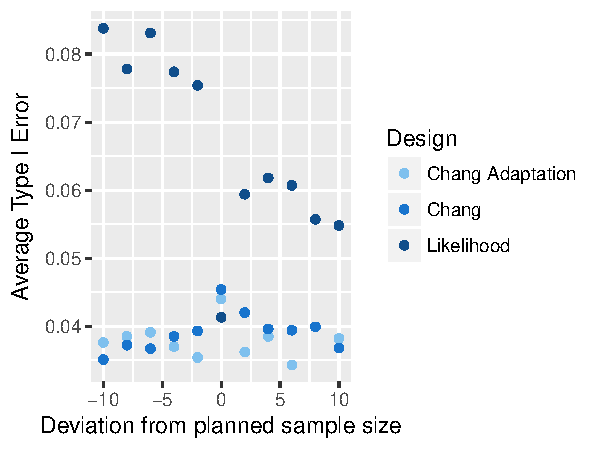
\includegraphics{unnamed-chunk-6-1} }

\end{Schunk}
\end{figure}

\begin{figure}[H]
\caption{Monte Carlo Simulation of Average Type I Error Rates of 20 Simon-like Designs when Stage I Sample Size Deviates from Planned for Attained Designs}
\begin{Schunk}


\centerline{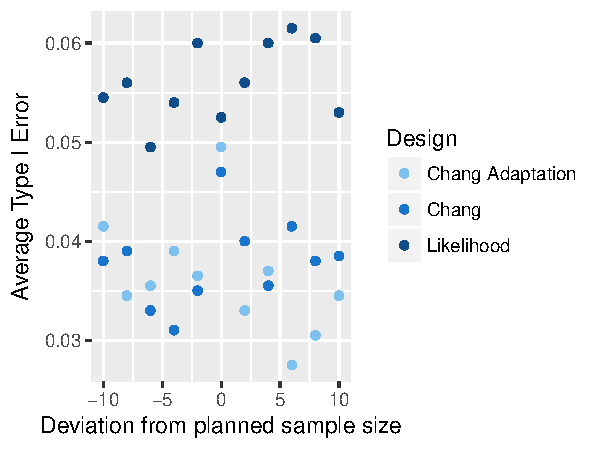
\includegraphics{unnamed-chunk-7-1} }

\end{Schunk}
\end{figure}



The findings will be put here - primarily tables covering different combinations of Simon's designs and unplanned sample sizes. 
\newline
Should maybe talk about how I couldn't replicate some results in the paper. 
\newline
Some differences with the likelihood: \\
controlling type 1 error, but criteria is controlling PET - I think T1E will still be controlled. Assuming stage II sample size and R2 is the same. We can add cohorts at the end of stage II. Talk about this.   \\


%%%%%%%%%%%%%%%%%%%%%%%%%%%%%%%%%%%%%%%%%%%%%%%%%%%%%%%%%%%%%%
%----------------Discussion--------------------------------%
%%%%%%%%%%%%%%%%%%%%%%%%%%%%%%%%%%%%%%%%%%%%%%%%%%%%%%%%%%%%%%
\section{Discussion}
\begin{itemize}
  \item Numerical study shows that keeping nt the same as the original has better properties.
  \item Talk about when the adaptation design and chang design will differ. (extreme sample size shifts? I cant remember.)
  \item Compare the design approaches
\end{itemize}


%%%%%%%%%%%%%%%%%%%%%%%%%%%%%%%%%%%%%%%%%%%%%%%%%%%%%%%%%%%%%%
%-----------------Appendix-------------------------------%
%%%%%%%%%%%%%%%%%%%%%%%%%%%%%%%%%%%%%%%%%%%%%%%%%%%%%%%%%%%%%%
\section{Appendix}
Maybe put the chang design here that goes beyond stage 2 sample size being origianl total and original second stage?



%%%%%%%%%%%%%%%%%%%%%%%%%%%%%%%%%%%%%%%%%%%%%%%%%%%%%%%%%%%%%%
%------------------Questions------------------------------%
%%%%%%%%%%%%%%%%%%%%%%%%%%%%%%%%%%%%%%%%%%%%%%%%%%%%%%%%%%%%%%
\section{Questions}

\begin{itemize}
  \item Particularly when describing other peoples' methods, how do you cite?
  \item If likelihood design can translate into simon's design and have better properties - can that be used as a tool to come up with these designs instead of using Chang's method? Or are they different because you're operating under frequentist vs likelihood inference? 
  \item Why do we choose PET closest to the original? - consider choosing closest PET, being conservative. mention that there are two ways to think about it. one is conservative and one is closest and they're pretty close to each other. 
\end{itemize}

\section{Notes}
\begin{itemize}
  \item inference from likelihood is more straightforward. the authors in koyama have shown that the p-value depends on the design. p-value's in multistage designs depend on the p-value. first stage is more complex. 
\end{itemize}
%%%%%%%%%%%%%%%%%%%%%%%%%%%%%%%%%%%%%%%%%%%%%%%%%%%%%%%%%%%%%%
%------------------------------------------------%
%%%%%%%%%%%%%%%%%%%%%%%%%%%%%%%%%%%%%%%%%%%%%%%%%%%%%%%%%%%%%%

%%%%%%%%%%%%%%%%%%%%%%%%%%%%%%%%%%%%%%%%%%%%%%%%%%%%%%%%%%%%%%
%-------------- BIBLIOGRAPHY--------------------------------------%
%%%%%%%%%%%%%%%%%%%%%%%%%%%%%%%%%%%%%%%%%%%%%%%%%%%%%%%%%%%%%%


%\bibliographystyle{apacite}
\bibliographystyle{ieeetr}
\bibliography{/Users/mollyolson/Documents/Vanderbilt/Masters_Thesis/ThesisRepo/thesisBib}		

\end{document} 


